
\documentclass[a4paper, 10pt]{article}  

\usepackage{geometry}
\geometry{a4paper, margin=1in}
    
    
\usepackage{verbatim}
\usepackage{graphicx}
\usepackage{pdfpages}
\usepackage{cite}
\usepackage{listings}
\usepackage{float}

\lstset{
	tabsize=2,
	breaklines=true
}

\setlength{\parskip}{1em}

\title{\LARGE \bf OpenCV Report 2\\Robotics and Automation  282 762}
\author{Marc Alexander Sferrazza \\ 12164165
\thanks{This work was not supported by any organization}
\thanks{Faculty of Mechatronics Engineering, Massey University, Albany, Auckland, New Zealand
        {\tt\small Progress of project: https://github.com/alex1v1a/Robotics-and-Automation/} } }

\begin{document}

\maketitle

\begin{figure}[H]
  
\includegraphics[width=\linewidth]{images/opencv}
  \label{fig:opencv}
\end{figure}

\thispagestyle{empty}
\pagestyle{plain}


%%%%%%%%%%%%%%%%%%%%%%%%%%%%%%%%%%%%%%%%%%%%%%%%%%%%%%%%%%%%%%%%%%%%%%%%%%%%%%%%

\begin{abstract}

A brief report on OpenCV object and colour detection. Each step was tested and an out image saved to the local folder when running the program to ensure a best rendered results, and easy debugging; these results can be tuned with the given functions in the program.

\end{abstract}


\clearpage
\tableofcontents
\thispagestyle{empty}
\clearpage

%%%%%%%%%%%%%%%%%%%%%%%%%%%%%%%%%%%%%%%%%%%%%%%%%%%%%%%%%%%%%%%%%%%%%%%%%%%%%%%%
%%%%%%%%%%%%%%%%%%%%%%%%%%%%%%%%%%%%%%%%%%%%%%%%%%%%%%%%%%%%%%%%%%%%%%%%%%%%%%%%

\setcounter{page}{1}

\section{INTRODUCTION}

OpenCV (Open Source Computer Vision Library) is an open source machine learning library for visual components. It has been widely accepted as one of the worlds most used image processing tools, and has the capability of static and dynamic comprehension. Some of the basic features available in OpenCV are capable mapping environments to be used in demonstration such as self driving cars lane detection. 

The process in this project to achieve is to design a program in the Visual Studio environment, using the OpenCV library that will detect an objects location and colour, in this case, red, blue, and yellow tennis balls. OpenCV is a powerful tool for image processing with more then 2500 algorithms available in its library; by using several functions within the OpenCV library, a processed image will produce these values. 

%%%%%%%%%%%%%%%%%%%%%%%%%%%%%%%%%%%%%%%%%%%%%%%%%%%%%%%%%%%%%%%%%%%%%%%%%%%%%%%%
%%%%%%%%%%%%%%%%%%%%%%%%%%%%%%%%%%%%%%%%%%%%%%%%%%%%%%%%%%%%%%%%%%%%%%%%%%%%%%%%

\section{METHOD}

An image has been provided of different colour tennis balls on a table. The process will involve filtering this image to a workable standard in which detection can be made of the circular objects and their respected colours. 

As there are five images the option to run the process with all outputs was first made, but then the decision of what images to check was implemented using the case keys 1, 2, 3, 4, 5, esc - A prompt will be given to the user to select which image to process and find the balls with their colours; the user can cycle back to the main image selection and select another image to process. The program can be closed by selecting the esc key from the prompt menu. The image is then loaded to memory and with each step through the detection the image is saved for easy debugging.  

After the user has selected a desired image to process the location function is called to preform the action. The sequence begins with the original image as shown below (set one from the five images are used for demo purposes in this report)

\begin{figure}[H]
  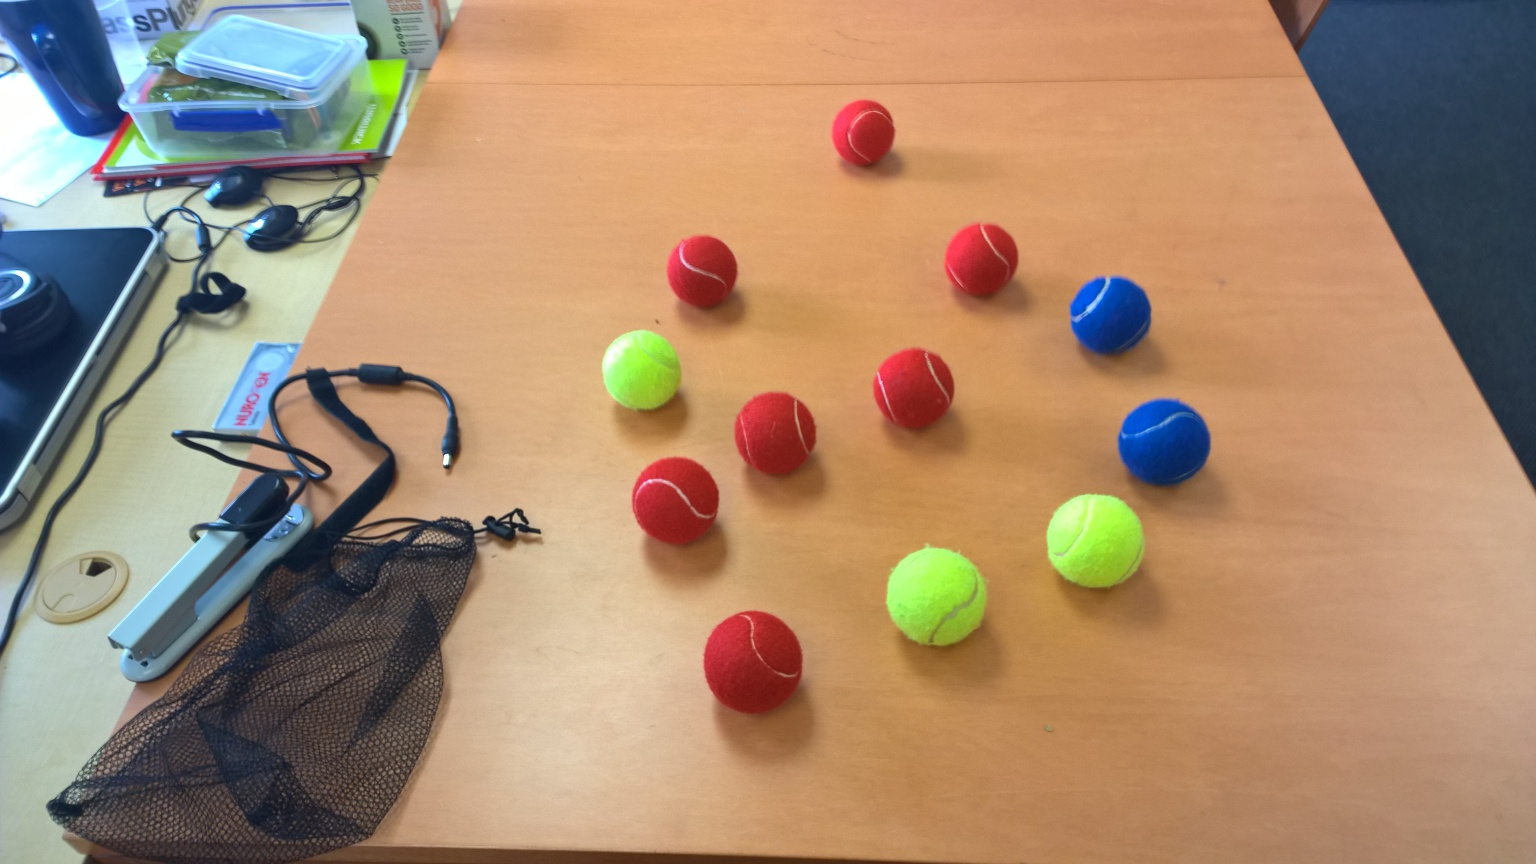
\includegraphics[width=\linewidth]{images/1}
  \caption{Original Image}
  \label{fig:Original Image}
\end{figure}

\clearpage
A full break down of the process has been attached and can be found in the code in the appendix. The following code is the process for user input and the function call for location.

\
\begin{lstlisting}[language = C++]
int main() {
	cout << "Choose an image to locate the tennis ball: 1, 2, 3, 4, 5...\n\npress esc to quit\n\n-------------------------------------------------------------------------\n" << endl;
	while (1) {
		namedWindow("User Select", CV_WINDOW_AUTOSIZE);
		switch (waitKey(0)) {
		case 27: // Exit prompt "esc"
			return 0;
		case 49: // Image 1 selected
			setpoint = 1;
			name = "1.jpg";
			location();
			break;
		case 50: // Image 2 selected
			setpoint = 2;
			name = "2.jpg";
			location();
			break;
		case 51: // Image 3 selected
			setpoint = 3;
			name = "3.jpg";
			location();
			break;
		case 52: // Image 4 selected
			setpoint = 4;
			name = "4.jpg";
			location();
			break;
		case 53: // Image 5 selected
			setpoint = 5;
			name = "5.jpg";
			location();
			break;
		}
	}
	return 0;
}
\end{lstlisting}

%%%%%%%%%%%%%%%%%%%%%%%%%%%%%%%%%%%%%%%%%%%%%%%%%%%%%%%%%%%%%%%%%%%%%%%%%%%%%%%%
\clearpage
\subsection{BGR to HSV conversion}

After the location function has been called, the image is read into memory and resized for processing. The aspect ratio of the first image was different then the others so it has been scaled accordingly. Complications arose from background colours when a ball was near another similar colour object such as the ice cream container, cup and exercise book, which is why the range needed to be limited.

In order to make the process more definite a conversion to HSV is necessary, this will make the process more robust by converting a BGR; The 8 bit 3 colour channel is converted to the huge, saturation and value which can be analysed more specifically easier in the provided functions. The HSV conversion is ready to begin, using the cvtColor function to convert the image to HSV (BGR2HSV) will help in the detection processing; the image is then saved for debugging.

\begin{lstlisting}[language = C++]
	// Read the image to memory and resize
	image = imread(name);
	if (setpoint != 1) {
		resize(image, image, Size(), 0.3, 0.3);
	}
	// Note that the aspect ratio of image 1 is significantly different than the others, these values provide better results
	else if (setpoint = 1) {
		resize(image, image, Size(), 0.5, 0.5);
	}

	// Copy origional image for end results edit
	imageFinal = image;

	// Step 1, Convert BGR to HSV
	cvtColor(image, hsv, COLOR_BGR2HSV);

	// After conversion save for reference
	//imshow("HSV", hsv); //Debugging feature
	nameh << namehsv << setpoint << ".jpg";
	imwrite(nameh.str(), hsv);
\end{lstlisting}

\begin{figure}[H]
  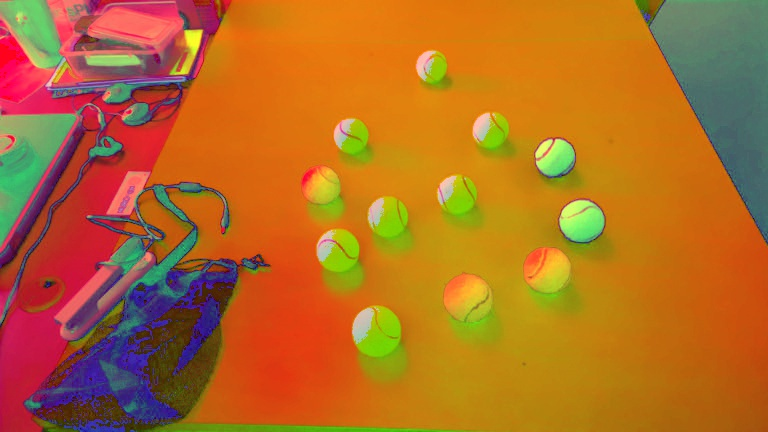
\includegraphics[width=\linewidth]{images/HSV}
  \caption{BGR to HSV conversion}
  \label{fig:BGR to HSV conversion}
\end{figure}

%%%%%%%%%%%%%%%%%%%%%%%%%%%%%%%%%%%%%%%%%%%%%%%%%%%%%%%%%%%%%%%%%%%%%%%%%%%%%%%%

\subsection{Thresholding}

When calculating the threshold, the range is found from the HSV image checking with 2 pass through arrays. The output will be a binary and help in detecting the edges of each ball like the first assignment with the canny function. As HSV has a specific range it is easily identifiable in each part however the image hue range (0-179) and saturation, value (0-255) may adjust with respect to lighting and depth, surrounding variables and factors to consider such as reflections and so on.

The array values given are scalar and are formed from the colours horizontal, vertical and scale values; when the range is found it writes to the output colour respectively then is added together and assigned to the image thres. Choosing only the selected colours we want from the image, yellow, red and blue; bearing in mind the hsv format of the image is the key step for this. 

The range and effected variables are difficult to establish, and while the paint colour detection tool is a standard feature on most computers nowadays it is not a practical method to address this solution; Luckily OpenCV provides a method to adjust these control levels to help find the limits for each image without too much fuss.

When preforming the tasks on each image the values may differ, therefore a multi-dimensional array has been set up to handle processing values for each image, making it simpler to process all the images in a more dynamic sense, these have been called through in different parts beginning here as the r-values. The rval's are read into each set of numeracies for the specific image when the location function is called, depending on what Image was chosen the corresponding pre-determined values are used. These have been found by using create trackers to measure the best values for high and low thresholds, hsv values, etc.

After the limits are found for the hsv for the tennis balls, the range limits are then set for thresholding. After each range has been completed the image will only show for that selected hsv value, so after finding the yellow, blue, and red ranges for the balls the image is merged to one range image with al there values; as the only known function to do this takes 2 arrays at a time the values are added twice.

\

\begin{lstlisting}[language = C++]
	// Step 2, Thresholding 
	// Check to find if arrays are in range
	Mat blue, red, yellow;
	inRange(hsv, Scalar(bHzLo, BSLow, bVrLo), Scalar(bHzHi, bScHi, bVrHi), blue);
	inRange(hsv, Scalar(rHzLo, RSLow, rVrLo), Scalar(rHzHi, rScHi, rVrHi), red);
	inRange(hsv, Scalar(yHzLo, yScLo, yVrLo), Scalar(yHzHi, yScHi, yVrHi), yellow);
	
	// Calculate the sum for 2 arrays twice 
	add(blue, red, thres);
	add(thres, yellow, thres);

	// After thresholding save for reference
	//imshow("Thresholding", thres); //Debugging feature
	namet << namethres << setpoint << ".jpg";
	imwrite(namet.str(), thres);
\end{lstlisting}

\begin{figure}[H]
  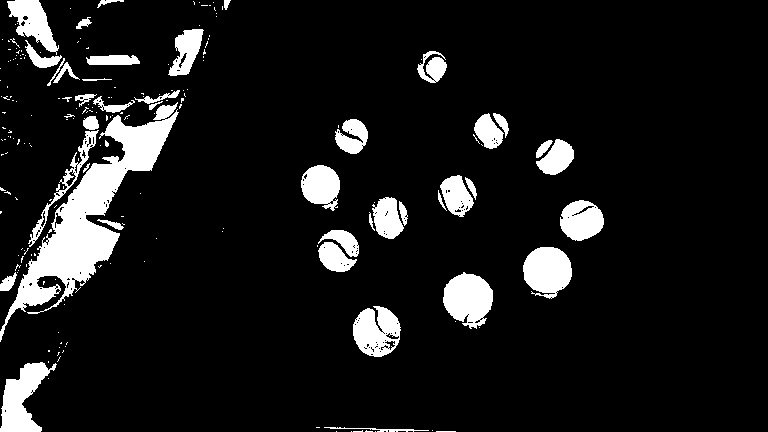
\includegraphics[width=\linewidth]{images/Thresholding}
  \caption{The process effect of thresholding}
  \label{fig:The process effect of thresholding}
\end{figure}

%%%%%%%%%%%%%%%%%%%%%%%%%%%%%%%%%%%%%%%%%%%%%%%%%%%%%%%%%%%%%%%%%%%%%%%%%%%%%%%%

\subsection{Dilation \& Erosion}

Using the dilation function the image begins to form more solid shapes and removes discrepancies to better form solid filled in shapes, by adding pixels to the boundaries found of objects and shapes in a greyscale image. The erosion function then emphasises those shapes making it easier for the shape identifier later on by removing pixels from the boundaries of objects. The best values found for the size of the morphological operations are as shown below.

\begin{lstlisting}[language = C++]
	// Step 3, Dilation and errosion used for multi level channel processing 
	dilate(thres, dilation, getStructuringElement(MORPH_ELLIPSE, Size(11, 11)));
	erode(dilation, errosion, getStructuringElement(MORPH_ELLIPSE, Size(3, 3)));

	// After dilation save for reference
	//imshow("Dilation", dilation); //Debugging feature
	named << namedilation << setpoint << ".jpg";
	imwrite(named.str(), dilation);

	// After errosion save for reference
	//imshow("Errosion", errosion); //Debugging feature
	namee << nameerrosion << setpoint << ".jpg";
	imwrite(namee.str(), errosion);
\end{lstlisting}

\begin{figure}[H]
  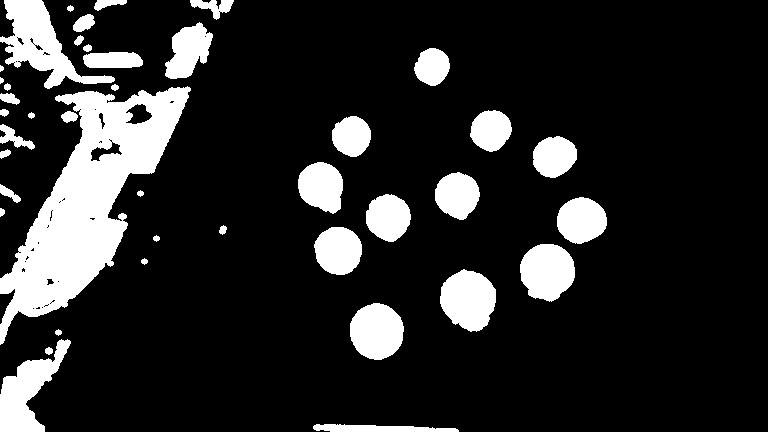
\includegraphics[width=\linewidth]{images/Dilation}
  \caption{The process effect of dilation}
  \label{fig:The process effect of dilation}
\end{figure}

\begin{figure}[H]
  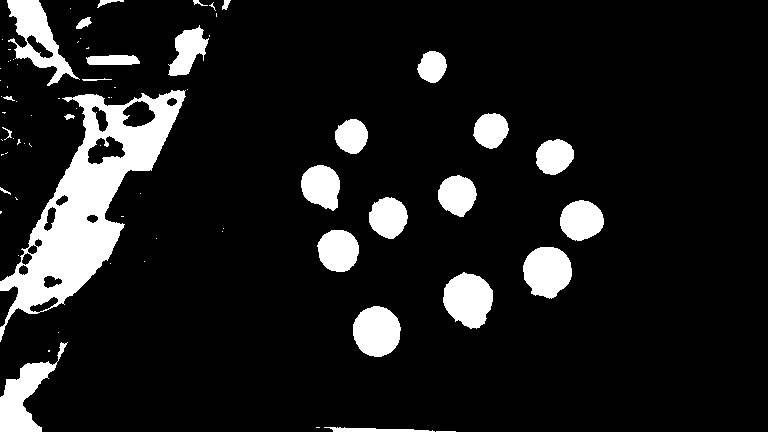
\includegraphics[width=\linewidth]{images/Erosion}
  \caption{The process effect of erosion}
  \label{fig:The process effect of erosion}
\end{figure}

%%%%%%%%%%%%%%%%%%%%%%%%%%%%%%%%%%%%%%%%%%%%%%%%%%%%%%%%%%%%%%%%%%%%%%%%%%%%%%%%
\clearpage
\subsection{Gaussian Blur}

The Gaussian blur is used to reduce the noise of the image and smoothing the edges to help eliminate any external influences when finding the shape and give a more accurate average of the pixels. The function will transform the image using convolution matrix Gaussian kernel, and will give a result based on each pixel and it's surrounding pixels to contour and blur while maintaining the edges integrity.

After the Gaussian process, the image is finally ready to be searched and labeled. The best values for the Gaussian have found to be a 7x7 kernel matrix with a 2.5 standard deviation. The image is saved for reference and then assigned to a new image for final searching and editing.

\begin{lstlisting}[language = C++]
	// Step 4, Preform Gaussian blur to further filter image and reduce noise to better detect the around point for the circles
	GaussianBlur(erosion, blur, Size(7, 7), 2.5, 2.5);

	// After Gaussian blur save for reference
	//imshow("Gaussian Blur", blur); //Debugging feature
	nameb << nameblur << setpoint << ".jpg";
	imwrite(nameb.str(), blur);		
\end{lstlisting}

\begin{figure}[H]
  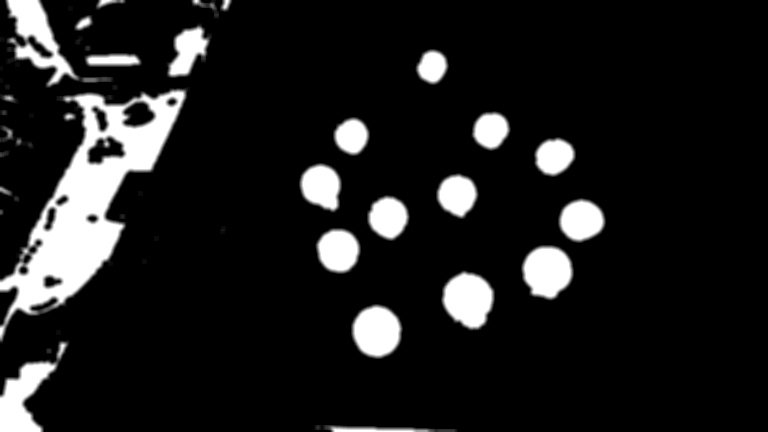
\includegraphics[width=\linewidth]{images/Blur}
  \caption{Noise reduction with Gaussian Blur}
  \label{fig:Noise reduction with Gaussian Blur}
\end{figure}

%%%%%%%%%%%%%%%%%%%%%%%%%%%%%%%%%%%%%%%%%%%%%%%%%%%%%%%%%%%%%%%%%%%%%%%%%%%%%%%%
\clearpage
\subsection{Hough Circles and Region of Interest}

Using the HoughCircles function to properly identify the tennis ball radius and thus the position of the center points of each tennis ball. Originally the Blob function was used, however the Hough method gave better results as the edges were detected pixel by pixel around the edge of each ball. The Hough algorithm works by voting on the shapes found with the parameters space local maxima to find certain shapes, in this case a circle thus HoughCircles. The pass through variables to the function for any image is given as an 8 bit single channel (greyscale), an output 3 element float vector with position and radius, the inverse ratio of the accumulator resolution to image resolution for this example being half. The minimum distance between each circle which changes depending on the image, the high and low threshold values typically being scaled by 3 from each other with the lower bing more sensitive to edges and in turn allowing more detection of possible shapes; the final parameters are the minimum and maximum circle radius.

Complications arose from background colours when a ball was near another similar colour object such as the ice cream container, cup and exercise book. The problem was looked at but a solution for distinguishing these objects from one another could not be established without partial circle, or more specific shadow filtering with correct proportion size. There is lots of noise on the left of the image due to some regions and the similar colours or threshold values, unfortunately it is unable to automatically ignore this sector so to simply cut it out the region of interest is set so only the tennis balls in this sector (the table) are recognised. 

A loop is then preformed to import the coordinates of the circles to location and colour matching, then the pixels are averaged from the surrounding pixels to assess the correct colour of each ball to match the colour to the positions.

\begin{lstlisting}[language = C++]
	// Step 5, Using the HoughCircles function to identify the tennis ball radius
	// Originally used the Blob function however this method gave better results
	HoughCircles(readyImage, ball, CV_HOUGH_GRADIENT, 2, dis, hThres, lThres, minRad, maxRad);
	for (size_t k = 0; k < ball.size(); k++) {
		Point center(cvRound(ball[k][0]), cvRound(ball[k][1]));
		// Establish and mark the center points
		int y = center.y, x = center.x;
		
		// Step 6, Meeting the criteria for the region of interest, ignore rest
		if ((roiXmin < x) && (x < roiXmax) && (roiYmin < y) && (y < roiYmax)) {
			for (int m = x - 5; m < x + 5; m++) {
				for (int n = y - 5; n < y + 5; n++) {
					Vec3b colorr = imageFinal.at<Vec3b>(n, m);
					meanr.val[0] = (colorr.val[0] + meanr.val[0]) / 2;
					meanr.val[1] = (colorr.val[1] + meanr.val[1]) / 2;
					meanr.val[2] = (colorr.val[2] + meanr.val[2]) / 2;
				}
			}
\end{lstlisting}

%%%%%%%%%%%%%%%%%%%%%%%%%%%%%%%%%%%%%%%%%%%%%%%%%%%%%%%%%%%%%%%%%%%%%%%%%%%%%%%%
\clearpage
\subsection{Labelling the targets found}

After looping through and finding all positions and colours the tennis balls are now ready for labelling. The putText and circle functions are used to briefly label each tennis balls center point, outer path and defined colour red, yellow, or blue. The coordinates are stored with the vec3f for reference so that only the colour referencing needs access to write the placements. Due to the enclosing area having breaks the average area of the ball is counted for the placement only, this means it will ignore then lines on the ball and take the basic shape.

The comparisons are made and the image is colour matched correctly with corresponding colours and locations, then the default drawing function is used to draw a circle enclosing the ball. The colours enclosing and text will match each tennis ball.

\begin{lstlisting}[language = C++]
			// Step 7, Font formatting and placement, standard fonts origionating from center point of each ball
			// Marking of each ball with center points
			int font = FONT_HERSHEY_SIMPLEX, thick = 1;
			float scale = 0.5;
			Point org(x, y);
			string colour;

			int radius = int(ball[k][2]);
			if ((meanr.val[0] > b1 && meanr.val[1] < b2 && meanr.val[2] < b3)
				|| (meanr.val[0] == 1 && meanr.val[1] == 252 && meanr.val[2] == 251)) {
				// Label each target found
				colour = "Blue";
				putText(imageFinal, colour, org, font, scale, Scalar(255, 0, 0), thick, 5);
				// Highlight each target with designating colour and mark the center points
				circle(imageFinal, center, radius, Scalar(255, 0, 0), 0, 5, 0);
				circle(imageFinal, center, 3, Scalar(255, 0, 0), 0, 5, 0);
			}
			if (meanr.val[0] < y1 && meanr.val[1] > y2 && meanr.val[2] > y3
				&& (meanr.val[0] != 1 && meanr.val[1] != 252 && meanr.val[2] != 251)) {
				// Label each target found
				colour = "Yellow";
				putText(imageFinal, colour, org, font, scale, Scalar(0, 255, 255), thick, 5);
				// Highlight each target with designating colour and mark the center points
				circle(imageFinal, center, radius, Scalar(0, 255, 255), 0, 5, 0);
				circle(imageFinal, center, 3, Scalar(0, 255, 255), 0, 5, 0);
			}			
			if (meanr.val[0] < r1 && meanr.val[1] < r2 && meanr.val[2] > r3) {
				// Label each target found
				colour = "Red";
				putText(imageFinal, colour, org, font, scale, Scalar(0, 0, 255), thick, 5);
				// Highlight each target with designating colour and mark the center points
				circle(imageFinal, center, radius, Scalar(0, 0, 255), 0, 5, 0);
				circle(imageFinal, center, 3, Scalar(0, 0, 255), 0, 5, 0);
			}
		}
	}

\end{lstlisting}


%%%%%%%%%%%%%%%%%%%%%%%%%%%%%%%%%%%%%%%%%%%%%%%%%%%%%%%%%%%%%%%%%%%%%%%%%%%%%%%%
%%%%%%%%%%%%%%%%%%%%%%%%%%%%%%%%%%%%%%%%%%%%%%%%%%%%%%%%%%%%%%%%%%%%%%%%%%%%%%%%
\clearpage

\section{RESULTS}

After the processing is complete the original image is displayed with the labels for each tennis ball found. The final result is shown below, the process is now successfully completed and the demonstration is complete. The user can now press any key to go back and select another image, or after closing the image hit the "esc" key to exit the program.

A sample of the results can be seen below.

\begin{lstlisting}[language = C++]
	cout << "Congradulations! Processing complete here are the tennis balls found with their respected colours!\n\npress any key to go back to main menu, or hit esc twice to quit\n\n-------------------------------------------------------------------------\n" << endl;
	// Step 8, After processing and locating tennis balls and colours complete, display final results, and save for reference
	namer << nameready << setpoint << ".jpg";
	imwrite(namer.str(), imageFinal);
	imshow(name, imageFinal); 
	// Wait for key press before returning to main menu
	waitKey(0);
	destroyAllWindows();
\end{lstlisting}

\begin{figure}[H]
  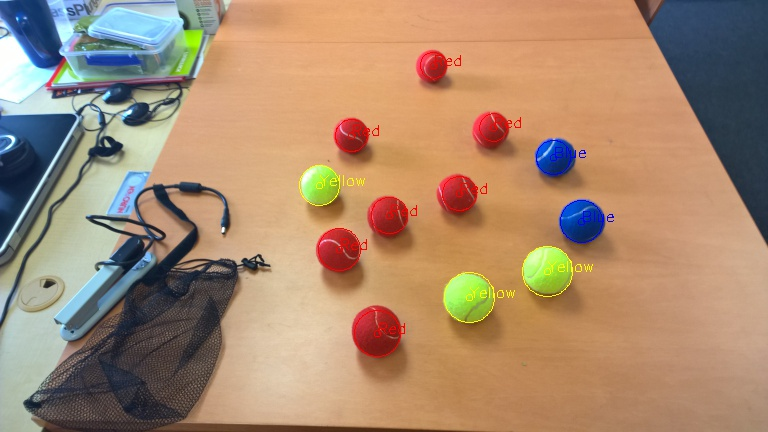
\includegraphics[width=\linewidth]{images/Final}
  \caption{The final image is given with detected results}
  \label{fig:The final image is given with detected results}
\end{figure}


%%%%%%%%%%%%%%%%%%%%%%%%%%%%%%%%%%%%%%%%%%%%%%%%%%%%%%%%%%%%%%%%%%%%%%%%%%%%%%%%

\subsection{Fine Tuning} 

While the process is straight forward and consists of step by step operations, the procedure in which required fine tuning. This involves checking the matrix at different points like the threshold values, dilation and erosion, the Gaussian blur, as well as the HoughCircles and region of interest.

The specific values were fiddled with to find the best combination and then tested.

%%%%%%%%%%%%%%%%%%%%%%%%%%%%%%%%%%%%%%%%%%%%%%%%%%%%%%%%%%%%%%%%%%%%%%%%%%%%%%%%
\clearpage
\subsection{Testing}

Ensure the target of finding the location of every tennis ball in each image is achieved, and that the colour of each ball is given.

Each step has an output image saved to check the processes respectively. The images are checked to make sure each stage is completing the task correctly, if not the code is then referred to and further revisions are made.

Every image was tested with the values for recognition and tweaked in the fine tuning process to get the best possible results.


%%%%%%%%%%%%%%%%%%%%%%%%%%%%%%%%%%%%%%%%%%%%%%%%%%%%%%%%%%%%%%%%%%%%%%%%%%%%%%%%

\subsection{Finalising}

Making the program stable and concise, and as robust as possible builds for a good design. Checking over the functions and any redundant code, ensure a good user interface is easily workable and the outputs are all correct.


%%%%%%%%%%%%%%%%%%%%%%%%%%%%%%%%%%%%%%%%%%%%%%%%%%%%%%%%%%%%%%%%%%%%%%%%%%%%%%%%
%%%%%%%%%%%%%%%%%%%%%%%%%%%%%%%%%%%%%%%%%%%%%%%%%%%%%%%%%%%%%%%%%%%%%%%%%%%%%%%%
\section{CONCLUSIONS}

The final detection of the tennis balls has been produced from several steps. This method provides basic filtering similar to that from assignment one before the processing locations are to be found. The filtering is to provide more accurate and stable results, and the HoughCircles detection was found better then the Blob function when tested. There were still some discrepancies with the output when processing the tennis balls with similar colour backgrounds.

The object detection was a success in sense but limited to that of this projects constraints. To better match solutions in the real world further algorithms would need to be acquired that are higher in focus, resolution, and more adaptive with environmental features for dynamic or moving objects with changing scenery and backgrounds, or if the camera is moving also.

%%%%%%%%%%%%%%%%%%%%%%%%%%%%%%%%%%%%%%%%%%%%%%%%%%%%%%%%%%%%%%%%%%%%%%%%%%%%%%%%
%%%%%%%%%%%%%%%%%%%%%%%%%%%%%%%%%%%%%%%%%%%%%%%%%%%%%%%%%%%%%%%%%%%%%%%%%%%%%%%%

\nocite{*}
\bibliographystyle{ieeetr}
\bibliography{references}

%%%%%%%%%%%%%%%%%%%%%%%%%%%%%%%%%%%%%%%%%%%%%%%%%%%%%%%%%%%%%%%%%%%%%%%%%%%%%%%%
%%%%%%%%%%%%%%%%%%%%%%%%%%%%%%%%%%%%%%%%%%%%%%%%%%%%%%%%%%%%%%%%%%%%%%%%%%%%%%%%

\clearpage
\section*{APPENDIX}

\begin{lstlisting}[language = C++]
// Marc Alexander Sferrazza 12164165
// Referenceing from http://docs.opencv.org/2.4/

#include <opencv2\opencv.hpp>
#include <opencv2\core.hpp>
#include <opencv2\imgcodecs.hpp>
#include <opencv2\highgui.hpp>
#include <iostream>
#include <string>
#include <stdio.h>
#include <stdlib.h>
#include <sstream>

using namespace cv;
using namespace std;

void location();

int setpoint;
string name;

int main() {
	cout << "Choose an image to locate the tennis ball: 1, 2, 3, 4, 5...\n\npress esc to quit\n\n-------------------------------------------------------------------------\n" << endl;
	while (1) {
		namedWindow("User Select", CV_WINDOW_AUTOSIZE);
		switch (waitKey(0)) {
		case 27: // Exit prompt "esc"
			return 0;
		case 49: // Image 1 selected
			setpoint = 1;
			name = "1.jpg";
			location();
			break;
		case 50: // Image 2 selected
			setpoint = 2;
			name = "2.jpg";
			location();
			break;
		case 51: // Image 3 selected
			setpoint = 3;
			name = "3.jpg";
			location();
			break;
		case 52: // Image 4 selected
			setpoint = 4;
			name = "4.jpg";
			location();
			break;
		case 53: // Image 5 selected
			setpoint = 5;
			name = "5.jpg";
			location();
			break;
		}
	}
	return 0;
}

void location() {
	Mat image, hsv, thres, dilation, errosion, blur, readyImage, imageFinal;
	
	int yHzLo, yHzHi, yScLo, yScHi, yVrLo, yVrHi;
	int rHzLo, rHzHi, RSLow, rScHi, rVrLo, rVrHi;
	int bHzLo, bHzHi, BSLow, bScHi, bVrLo, bVrHi;
	int roiXmin, roiXmax, roiYmin, roiYmax;
	int r1, r2, r3, b1, b2, b3, y1, y2, y3;
	int hThres, lThres, dis, minRad, maxRad;

	// Naming the saved output files for reference
	ostringstream nameh, namet, named, namee, nameb, namer;
	string namehsv, namethres, namedilation, nameerrosion, nameblur, nameready;
	// Image save locations
	namehsv = "Output/1.HSV Image ";
	namethres = "Output/2.Thresholding Image ";
	namedilation = "Output/3.Dilation Image ";
	nameerrosion = "Output/4.Errosion Image ";
	nameblur = "Output/5.GaussianBlur Image ";
	nameready = "Output/6.Final Result Image ";

	// Read the image to memory and resize
	image = imread(name);
	if (setpoint != 1) {
		resize(image, image, Size(), 0.3, 0.3);
	}
	// Note that the aspect ratio of image 1 is significantly different than the others, these values provide better results
	else if (setpoint = 1) {
		resize(image, image, Size(), 0.5, 0.5);
	}

	// Copy origional image for end results edit
	imageFinal = image;

	// Step 1, Convert BGR to HSV
	cvtColor(image, hsv, COLOR_BGR2HSV);

	// After conversion save for reference
	//imshow("HSV", hsv); //Debugging feature
	nameh << namehsv << setpoint << ".jpg";
	imwrite(nameh.str(), hsv);

	int rval[5][36] = {
		{ 31, 0, 142, 60, 255, 255, 0, 186, 69, 179, 213, 255, 53, 206, 51, 179, 255, 255, 300, 700, 50, 470, 100, 100, 100, 90, 50, 30, 100, 100, 100, 150, 50, 30, 10, 40 },
		{ 153, 148, 128, 179, 227, 255, 90, 121, 0, 114, 255, 255, 22, 63, 148, 89, 198, 255, 260, 700, 170, 470, 110, 100, 100, 100, 130, 50, 140, 180, 110, 150, 50, 30, 10, 40 },
		{ 21, 142, 146, 43, 255, 255, 0, 148, 75, 7, 255, 255, 92, 178, 8, 150, 255, 225, 260, 700, 50, 470, 50, 40, 70, 20, 30,20, 10, 160, 160, 126, 42, 30, 5, 40 },
		{ 18, 194, 57, 35, 255, 255, 0, 190, 69, 6, 255, 255, 107, 176, 45, 112, 255, 255, 260, 700, 50, 470, 60, 65, 67, 34, 85, 88, 100, 100, 100, 82, 34, 30, 10, 40 },
		{ 17, 190, 99, 49, 255, 255, 0, 144, 81, 8, 215, 190, 105, 168, 24, 157, 255, 204, 260, 600, 170, 470, 100, 100, 100, 66, 70, 61, 100, 100, 100, 100, 33, 30, 10, 40 }
	};

	int *propd[36] = {
		&yHzLo, &yScLo, &yVrLo, &yHzHi, &yScHi, &yVrHi,
		&rHzLo, &RSLow, &rVrLo, &rHzHi, &rScHi, &rVrHi,
		&bHzLo, &BSLow, &bVrLo, &bHzHi, &bScHi, &bVrHi,
		&roiXmin, &roiXmax, &roiYmin, &roiYmax,
		&r1, &r2, &r3, &b1, &b2, &b3, &y1, &y2, &y3,
		&hThres, &lThres, &dis, &minRad, &maxRad
	};

	// Set random numbers to the array
	for (int k = 0; k < 36; k++) {
		*propd[k] = rval[setpoint - 1][k];
	}

	// Step 2, Thresholding 
	// Check to find if arrays are in range
	Mat blue, red, yellow;
	inRange(hsv, Scalar(bHzLo, BSLow, bVrLo), Scalar(bHzHi, bScHi, bVrHi), blue);
	inRange(hsv, Scalar(rHzLo, RSLow, rVrLo), Scalar(rHzHi, rScHi, rVrHi), red);
	inRange(hsv, Scalar(yHzLo, yScLo, yVrLo), Scalar(yHzHi, yScHi, yVrHi), yellow);
	
	// Calculate the sum for 2 arrays twice 
	add(blue, red, thres);
	add(thres, yellow, thres);

	// After thresholding save for reference
	//imshow("Thresholding", thres); //Debugging feature
	namet << namethres << setpoint << ".jpg";
	imwrite(namet.str(), thres);

	// Step 3, Dilation and errosion used for multi level channel processing 
	dilate(thres, dilation, getStructuringElement(MORPH_ELLIPSE, Size(11, 11)));
	erode(dilation, errosion, getStructuringElement(MORPH_ELLIPSE, Size(3, 3)));

	// After dilation save for reference
	//imshow("Dilation", dilation); //Debugging feature
	named << namedilation << setpoint << ".jpg";
	imwrite(named.str(), dilation);

	// After errosion save for reference
	//imshow("Errosion", errosion); //Debugging feature
	namee << nameerrosion << setpoint << ".jpg";
	imwrite(namee.str(), errosion);

	// Step 4, Preform Gaussian blur to further bilter image and reduce noise to better detect the raound point for the circles
	GaussianBlur(errosion, blur, Size(7, 7), 2.5, 2.5);

	// After Gaussian blur save for reference
	//imshow("Gaussian Blur", blur); //Debugging feature
	nameb << nameblur << setpoint << ".jpg";
	imwrite(nameb.str(), blur);

	// Assign the filtered image to readyImage for location processing
	readyImage = blur;
	vector<Vec3f> ball;
	Vec3b meanr;

	// Step 5, Using the HoughCircles function to identify the tennis ball radius
	// Originally used the Blob function however this method gave better results
	HoughCircles(readyImage, ball, CV_HOUGH_GRADIENT, 2, dis, hThres, lThres, minRad, maxRad);
	for (size_t k = 0; k < ball.size(); k++) {
		Point center(cvRound(ball[k][0]), cvRound(ball[k][1]));
		// Establish and mark the center points
		int y = center.y, x = center.x;

		// Step 6, Meeting the criteria for the region of interest, ignore rest
		if ((roiXmin < x) && (x < roiXmax) && (roiYmin < y) && (y < roiYmax)) {
			for (int m = x - 5; m < x + 5; m++) {
				for (int n = y - 5; n < y + 5; n++) {
					Vec3b colorr = imageFinal.at<Vec3b>(n, m);
					meanr.val[0] = (colorr.val[0] + meanr.val[0]) / 2;
					meanr.val[1] = (colorr.val[1] + meanr.val[1]) / 2;
					meanr.val[2] = (colorr.val[2] + meanr.val[2]) / 2;
				}
			}

			// Step 7, Font formatting and placement, standard fonts origionating from center point of each ball
			// Marking of each ball with center points
			int font = FONT_HERSHEY_SIMPLEX, thick = 1;
			float scale = 0.5;
			Point org(x, y);
			string colour;

			int radius = int(ball[k][2]);
			if ((meanr.val[0] > b1 && meanr.val[1] < b2 && meanr.val[2] < b3)
				|| (meanr.val[0] == 1 && meanr.val[1] == 252 && meanr.val[2] == 251)) {
				// Label each target found
				colour = "Blue";
				putText(imageFinal, colour, org, font, scale, Scalar(255, 0, 0), thick, 5);
				// Highlight each target with designating colour and mark the center points
				circle(imageFinal, center, radius, Scalar(255, 0, 0), 0, 5, 0);
				circle(imageFinal, center, 3, Scalar(255, 0, 0), 0, 5, 0);
			}
			if (meanr.val[0] < y1 && meanr.val[1] > y2 && meanr.val[2] > y3
				&& (meanr.val[0] != 1 && meanr.val[1] != 252 && meanr.val[2] != 251)) {
				// Label each target found
				colour = "Yellow";
				putText(imageFinal, colour, org, font, scale, Scalar(0, 255, 255), thick, 5);
				// Highlight each target with designating colour and mark the center points
				circle(imageFinal, center, radius, Scalar(0, 255, 255), 0, 5, 0);
				circle(imageFinal, center, 3, Scalar(0, 255, 255), 0, 5, 0);
			}			
			if (meanr.val[0] < r1 && meanr.val[1] < r2 && meanr.val[2] > r3) {
				// Label each target found
				colour = "Red";
				putText(imageFinal, colour, org, font, scale, Scalar(0, 0, 255), thick, 5);
				// Highlight each target with designating colour and mark the center points
				circle(imageFinal, center, radius, Scalar(0, 0, 255), 0, 5, 0);
				circle(imageFinal, center, 3, Scalar(0, 0, 255), 0, 5, 0);
			}
		}
	}
	cout << "Congradulations! Processing complete here are the tennis balls found with their respected colours!\n\npress any key to go back to main menu, or hit esc twice to quit\n\n-------------------------------------------------------------------------\n" << endl;
	// Step 8, After processing and locating tennis balls and colours complete, display final results, and save for reference
	namer << nameready << setpoint << ".jpg";
	imwrite(namer.str(), imageFinal);
	imshow(name, imageFinal); 
	// Wait for key press before returning to main menu
	waitKey(0);
	destroyAllWindows();
}
\end{lstlisting}

\end{document}
